\documentclass{beamer}
\usepackage[latin1]{inputenc}
\usepackage{amsmath}
\usepackage{graphicx}
\usepackage{multimedia}
\usepackage{caption}
\usetheme{default}
\usecolortheme{default}
\definecolor{darkred}{RGB}{24,0,0}
\setbeamercolor{title}{fg=red}
\setbeamertemplate{blocks}[rounded][shadow=true]
\setbeamertemplate{itemize items}[square]
\usefonttheme{serif}
\title{\textbf{The effect of gas bulk rotation on the morphology of the Ly$\alpha$ line.}}
\author{Juan Nicol\'as Garavito-Camargo \\ Advisor: Jaime E. Forero-Romero}
\institute{Universidad de los Andes, Bogot\'a, Colombia}
\date{May 20, 2015}
\begin{document}

\begin{frame}
\titlepage
\author
\institute
\begin{figure}
%\rule{1.28cm}{0.72cm}
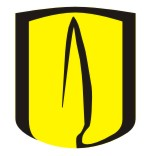
\includegraphics[scale=0.35]{Figures/logo.jpeg}
\end{figure}
\end{frame}


\begin{frame}{Lyman $\alpha$ emission line:}
A Ly$\alpha$ photon is emitted with a $\lambda= 121.56 nm$.
\begin{figure}
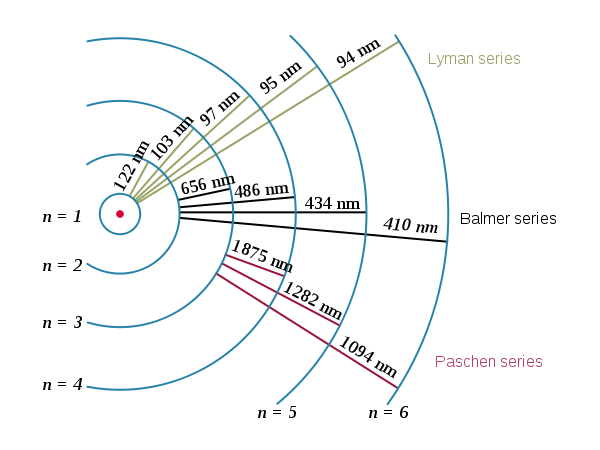
\includegraphics[scale=0.4]{Figures/Hydrogen_transitions.png}
\end{figure}
\end{frame}

\begin{frame}{Ly$\alpha$ is in the vacuum UV part of the EM spectrum}
\begin{figure}
\centering
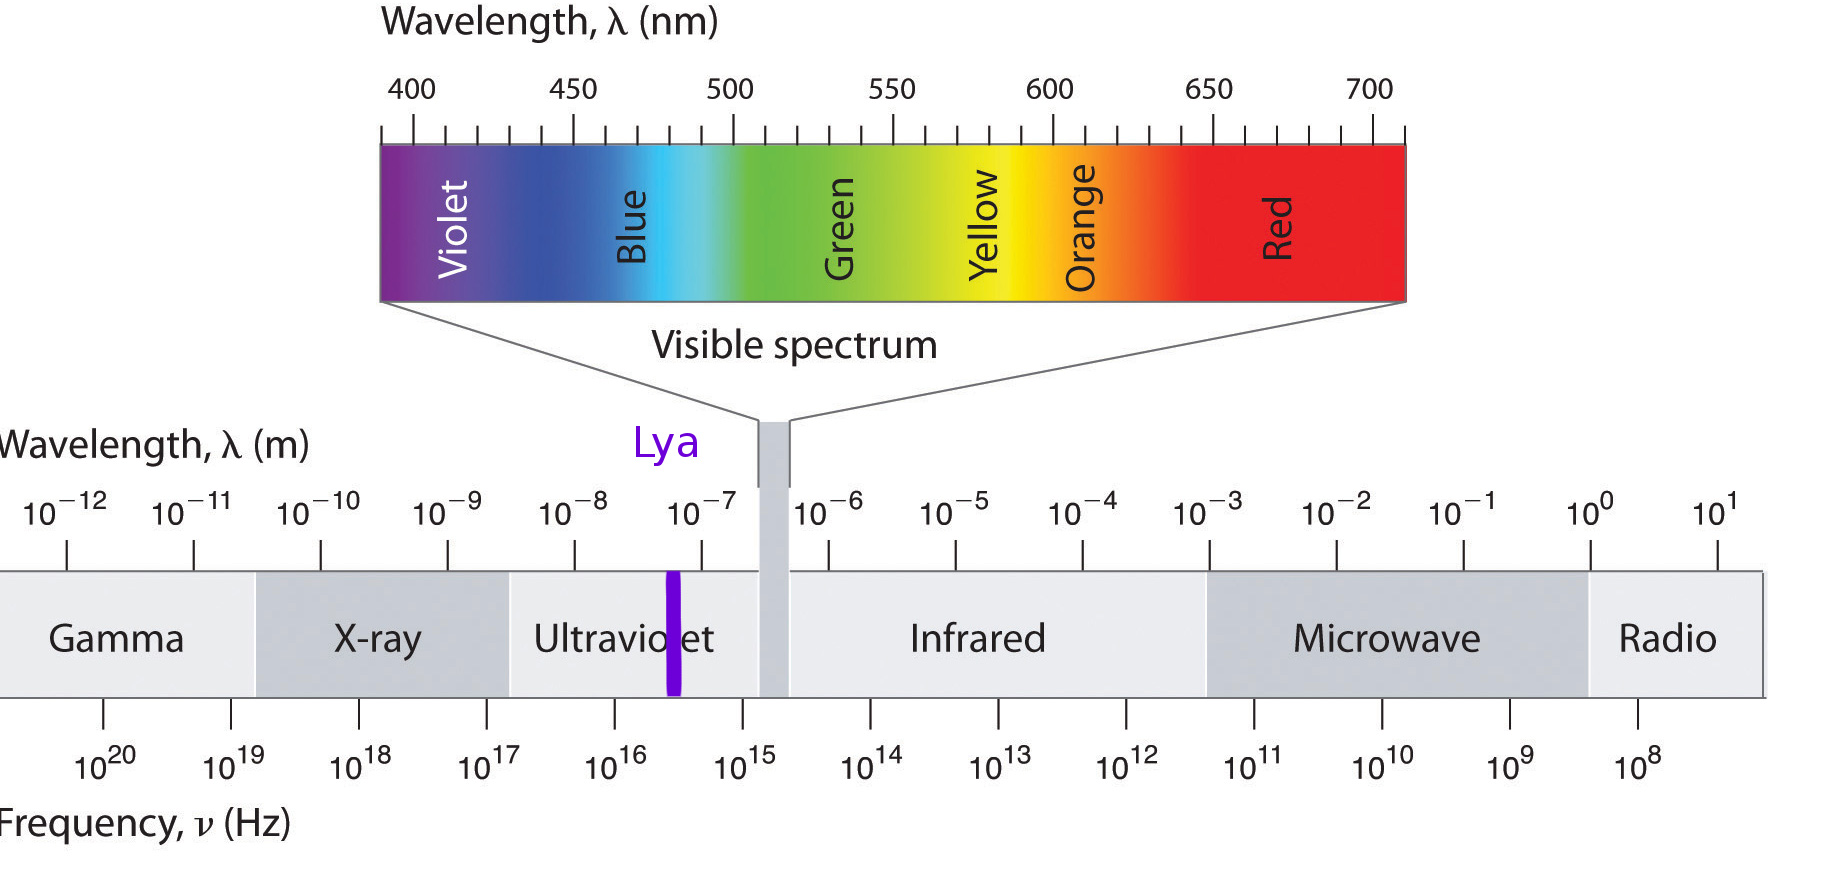
\includegraphics[scale=0.18]{Figures/em.jpg}
\end{figure}
\end{frame}


\begin{frame}
\begin{figure}
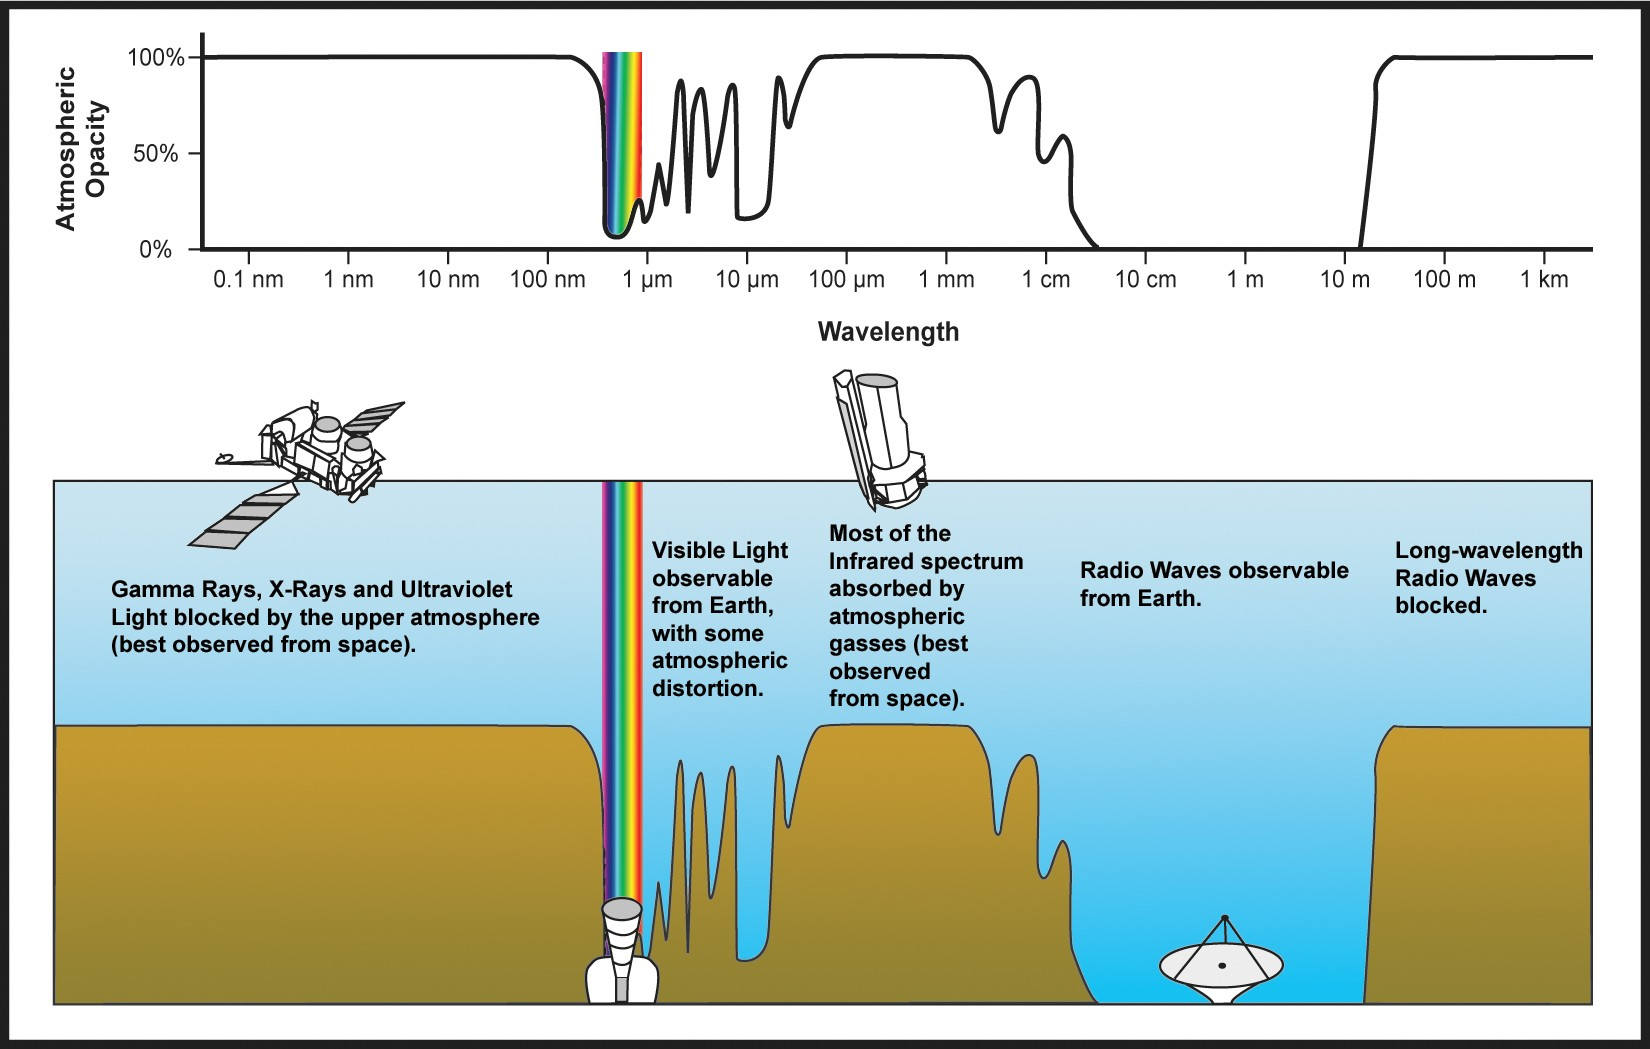
\includegraphics[scale=0.8]{Figures/AtmosphericEM.jpg}
\caption{Atmospheric radiation absorption}
\end{figure}
\end{frame}


%\begin{frame}
%Lya line characteristics
%\end{frame}

\begin{frame}{Cosmological Redshift \& the observable LAEs in the visible regime.}
\begin{figure}
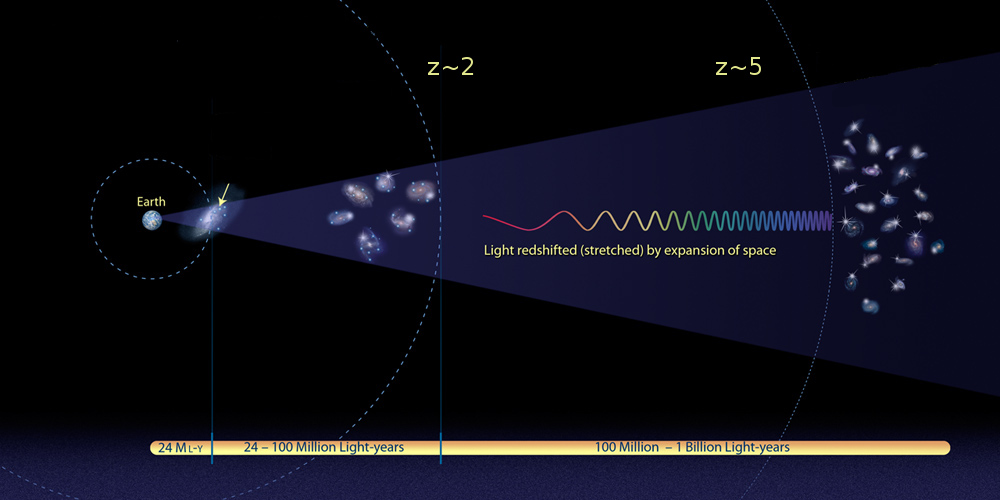
\includegraphics[scale=0.3]{Figures/expansion.jpg}
\caption{Image credit: NASA, ESA, and A. Feild (STScI).}
\end{figure}
\end{frame}

\begin{frame}
\begin{center}
\LARGE{Do galaxies radiate Ly$\alpha$ photons?}
\end{center}
\end{frame}

\begin{frame}{Hydrogen in the most abundant element in the Universe.} 
\begin{figure}
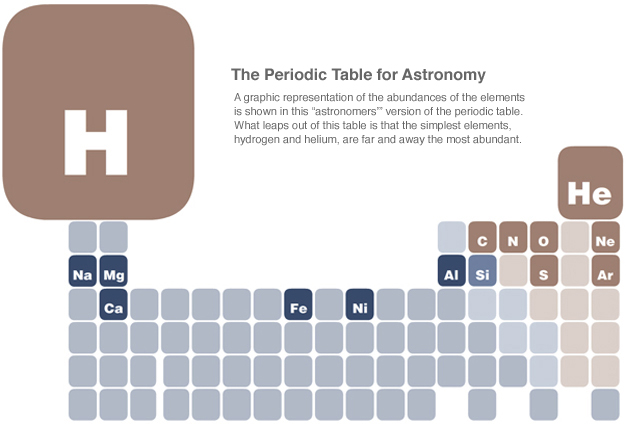
\includegraphics[scale=0.3]{Figures/astronomy_table.jpg}
\caption{Astronomers periodic table. Image credit: http://chandra.harvard.edu}
\end{figure}
\end{frame}

\begin{frame}{UV radiation mechanisms and sources:}

\begin{itemize}
\item UV stellar radiation 
\item Gravitational cooling
\item UV background radiation
\end{itemize}

\end{frame}

\begin{frame}%n{figure}
\begin{figure}
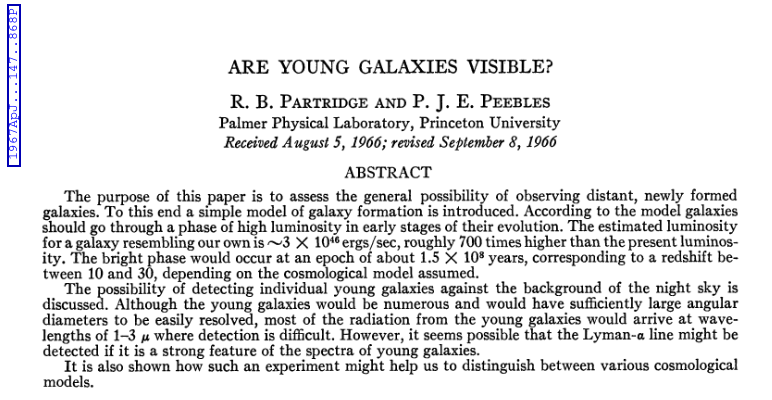
\includegraphics[scale=0.4]{Figures/PP.png}
\end{figure}
\end{frame}


\begin{frame}
\LARGE{25 years later ...}
\end{frame}

\begin{frame}
\begin{figure}
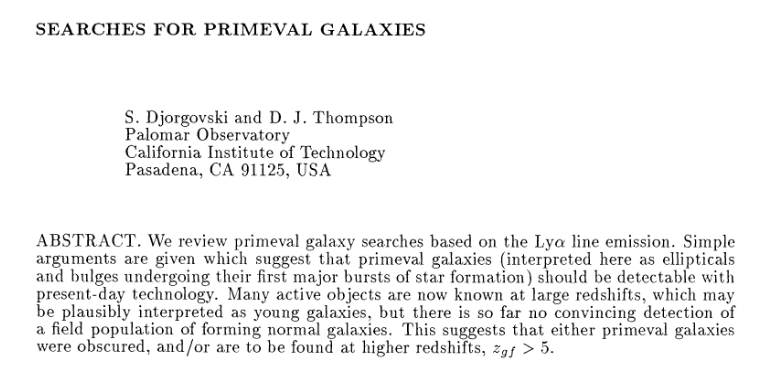
\includegraphics[scale=0.4]{Figures/DJT.png}
\end{figure}
\end{frame}

\begin{frame}{Ly $\alpha$ as an important tool in extragalactic astronomy}

\end{frame}

% units convention 
%\begin{frame}{Units convention:}
%\begin{equation}
%V = \dfrac{\nu_{obs} - \nu_{\alpha}}{c}
%\end{equation}
%\end{frame}

\begin{frame}{LAEs observed spectra:}
\begin{figure}
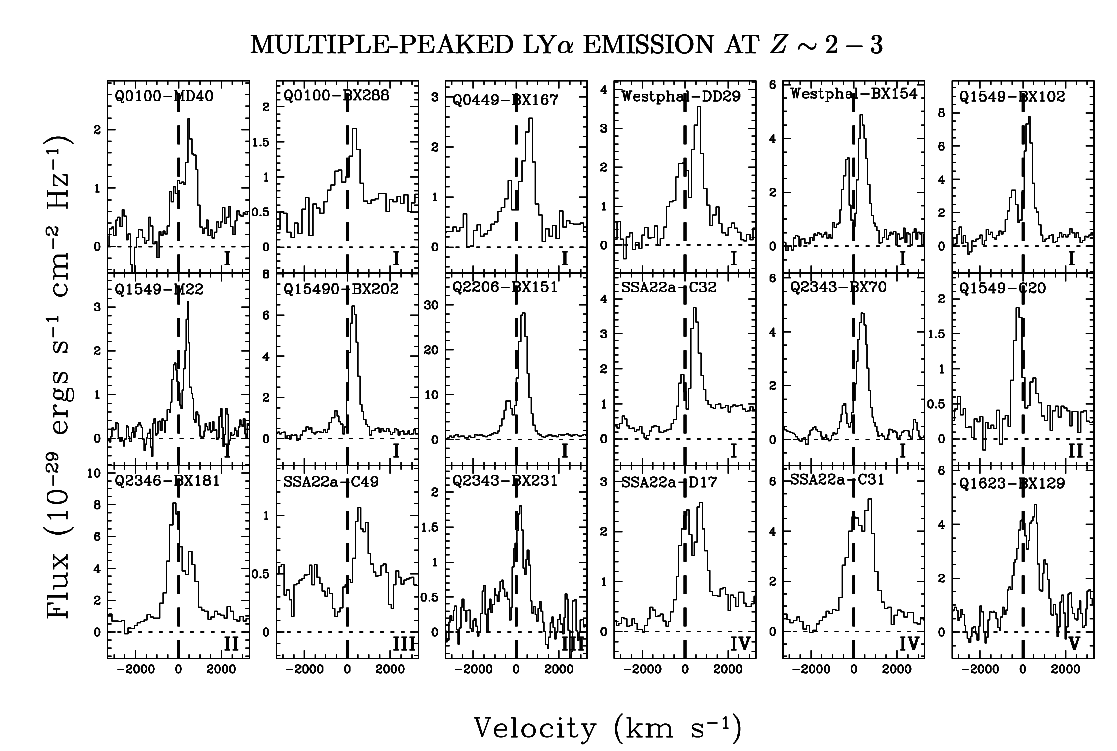
\includegraphics[scale=0.33]{Figures/kulas.png}
\caption*{Kulas e.a ApJ, 2012.}
\end{figure}
\end{frame}

\begin{frame}{Radiative transfer through a static medium:}
\begin{figure}
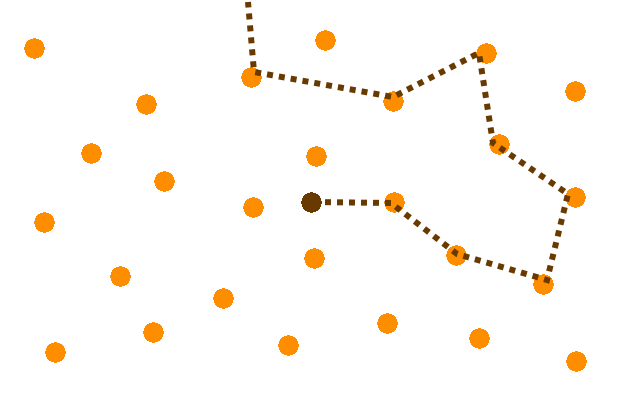
\includegraphics[scale=0.3]{Figures/RT.png}
\end{figure}
\end{frame}

\begin{frame}{Radiative transfer through a non-static medium:}
\begin{figure}
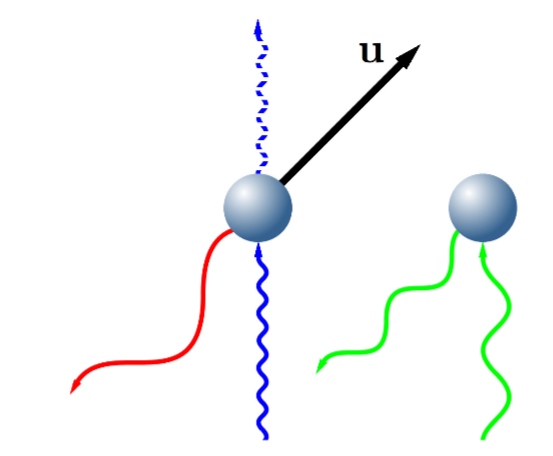
\includegraphics[scale=0.4]{Figures/xshift.png}
\end{figure}
\end{frame}


\begin{frame}{Ly$\alpha$ photons undergoes a random walk in space and wavelength}
\begin{figure}
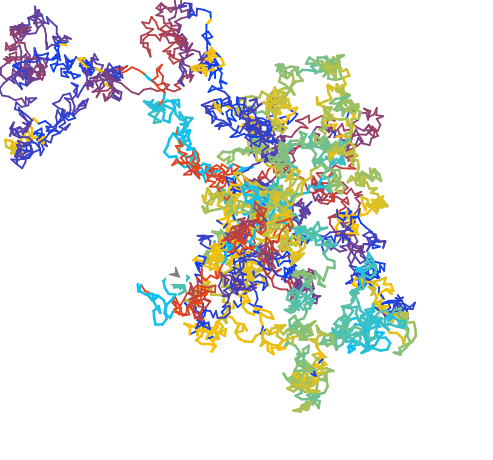
\includegraphics[scale=0.4]{Figures/rand_walk.png}
\end{figure}
\end{frame}

\begin{frame}{Dust and escape fraction of Ly$\alpha$ photons}
Dust grains can either absorve or scatter Ly$\alpha$ photons. The probability
of these events is given by the \textbf{Albedo (A)}.

\[   
A = \dfrac{\sigma_{scatt}}{\sigma_{dust}}
\]

The ratio of Ly$\alpha$ phtons observed over the Ly$\alpha$ photons emitted
define the \textbf{escape fracion $f_{esc}$}.
 
\end{frame}

\begin{frame}{Radiative transfer theory I:*}

\begin{equation}\label{eq:analytic}
\dfrac{d J(\nu)}{d\tau} = \dfrac{(\Delta \nu_D)^2}{2}\dfrac{\partial}{\partial \nu}\phi (\nu) \dfrac{\partial J(\nu)}{\partial \nu}
\end{equation}

Where $\nu$ is the frequency of the photons, $\phi(\nu)$ is the Voigt profile and $\tau$
the optical depth.

\begin{figure}
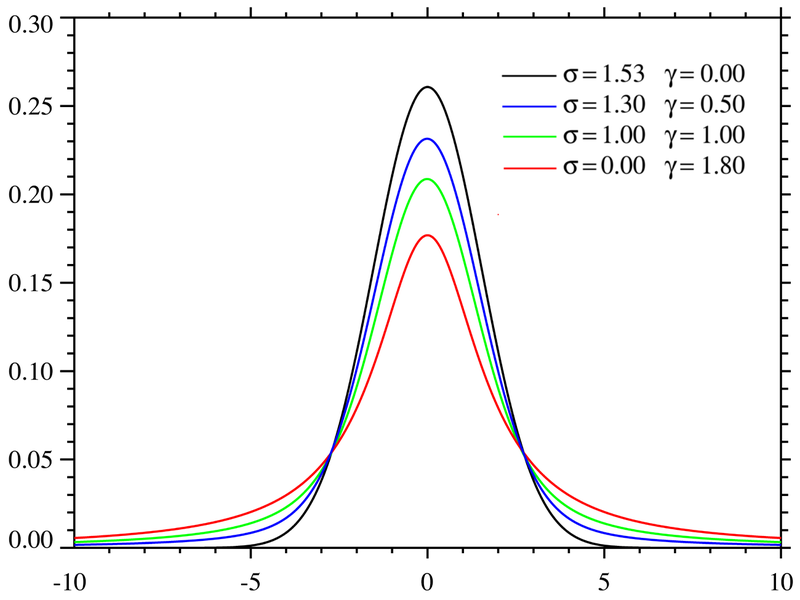
\includegraphics[scale=0.2]{Figures/voigt.png}
\caption{Voigt profile}
\end{figure}

\end{frame}

\begin{frame}{Analytical models}
The solution of Eq.\ref{eq:analytic} has been achieved for \textbf{two} simplified 
models: The infinite homogeneous slab and the homogeneous sphere, both with central 
Ly$\alpha$ sources.\\

This analytical solution for the slab geometry was derived by Neufeld in 1990.  

\begin{equation}
J(\tau, x) = \dfrac{\sqrt{6}}{24}\dfrac{x^2}{\sqrt{\pi}a \tau cosh[\sqrt{\pi^3/54}(x^3 - x_{in}^3)]}
\end{equation}

Where $a = A / 4\pi \Delta \nu_D$ is the voigt parameter and $\tau$ the optical depth. Harrington in 
1993 derived the frequency at which the line has the maximum intensity:

\[
x_m = \pm 1.066 (a\tau)^(1/3)
\]

And the average number of scatterings:

\[
N_{scatt} = 1.612 \tau
\]

\end{frame}

\begin{frame}{Infinite slab spectrum:}
\begin{figure}
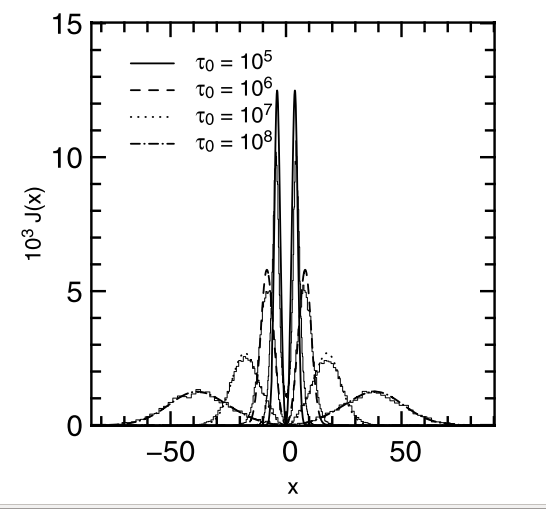
\includegraphics[scale=0.4]{Figures/slab.png}
\caption*{Forero-Romero e.a 2011.}
\end{figure}
\end{frame}


\begin{frame}{Homogeneous dustless sphere with central sources:}

Mark Dijkstra in 2006 has deirved the analytical profile of the dustless sphere with 
central sources. 

\begin{equation}
J(\tau, x) = \dfrac{\sqrt{\pi}}{4 \sqrt{6}} \dfrac{x^2}{a \tau (1 + cosh[\sqrt{2\pi^3/27}x^3 / a\tau])}
\end{equation}

\begin{figure}
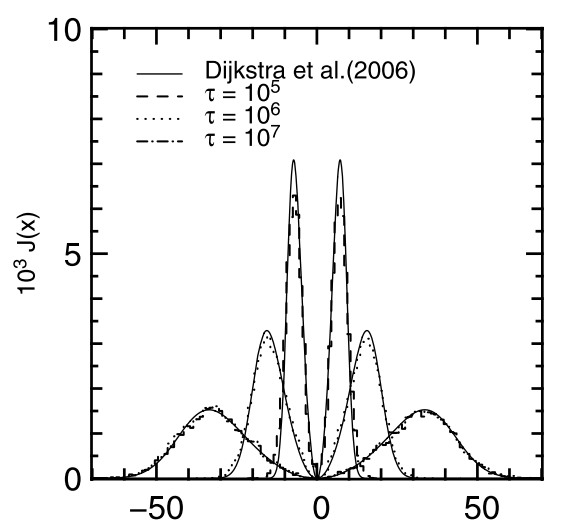
\includegraphics[scale=0.2]{Figures/sphere.png}
\caption*{Forero-Romero e.a 2011.}
\end{figure}
\end{frame}
%-------------------------- Previous studies ---------------------

\begin{frame}
\LARGE{Monte-Carlo approach:}
\end{frame}

\begin{frame}{Radiative Transfer via Monte-Carlo methods:}
\begin{itemize}
\item Set up the initial conditions (Temperature, gas distibution \& kinematics).
\item Set the Ly$\alpha$ photons initial positions $x_{in}$.
\item Generate the photon random displacement $\tau_0$ in a random direction
$\vec{n}$.
\item Derive the HI atom velocity components from the initial field and
generate random components for the thermal movements.
\item Set the new Ly$\alpha$ direction after the scattering.
\item Set the absorption probability due to dust encounters.
\item Iterate from step 2.
\end{itemize}
\end{frame}



\begin{frame}{Expanding/Contracting sphere:}
\begin{figure}
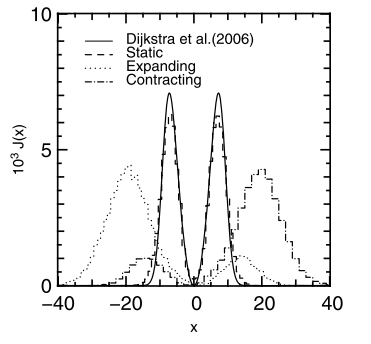
\includegraphics[scale=0.4]{Figures/expanding.png}
\end{figure}
\end{frame}

\begin{frame}{Cavities}
Zheng/Zheng and Dijkstra
\end{frame}

\begin{frame}{A SPH simulated galaxy spectrum}
\begin{figure}
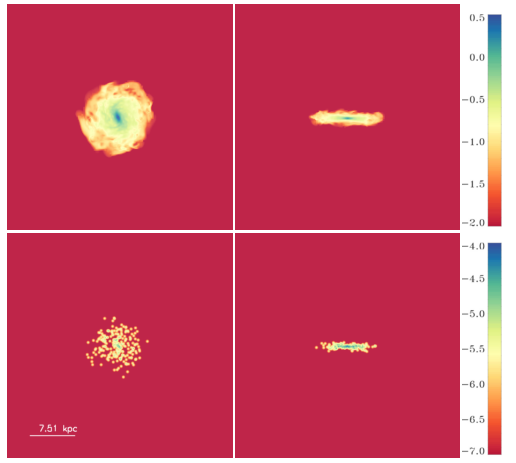
\includegraphics[scale=0.3]{Figures/verhamme1.png}
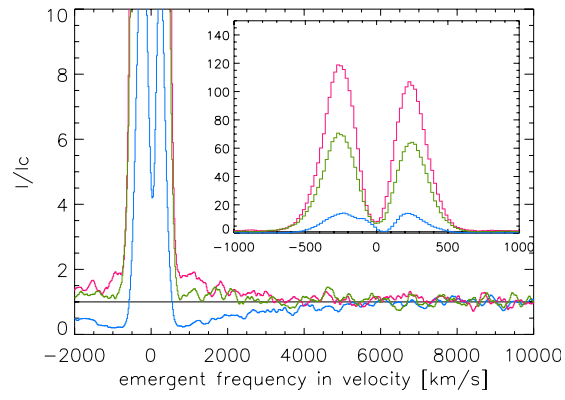
\includegraphics[scale=0.3]{Figures/Verhamme2.png}
\end{figure}
\end{frame}

\begin{frame}
\LARGE{Different geometries and kinematics of the gas have an impact on the morphology of the
Ly$\alpha$ spectrum.}\\

\end{frame}


%---------------------RESULTS-----------------------------

\begin{frame}
\LARGE{What would be the effect of roation on the morphology of the Ly$\alpha$ line ? 
Is this effect observable?} 
\end{frame}


\begin{frame}
\begin{figure}
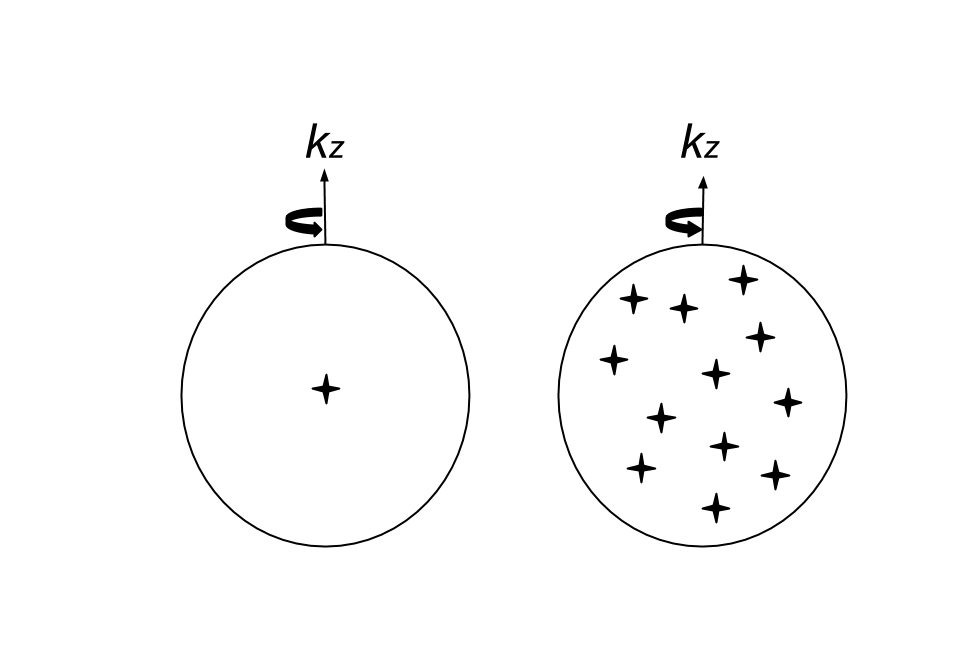
\includegraphics[scale=0.3]{Figures/models.png}
\end{figure}
\end{frame}

\begin{frame}{Models}
\begin{table}
\begin{center}
\begin{tabular}{llc}\hline\hline
Physical Parameter (units) & Symbol & Values\\\hline
Velocity ($km/s$) & $V_{\rm max}$&$0,\ \ 100,\ 200,\ 300$\\
Hydrogen Optical Depth & $\tau_{H} $ & $10^{5},\ 10^{6},\ 10^{7}$\\
Dust Optical Depth & $\tau_{a}$ & $0$,$1$\\
Photons Distributions & & Central, Homogeneous\\\hline\hline
\end{tabular}
\caption{Summary of Physical Parameters of our Monte Carlo Simulations.}
\end{center}
\end{table}
\end{frame}


\begin{frame}
\LARGE{We measure the impact of rotation and viewing angle $\theta$ for the 
main line characteristics.}
\begin{figure}
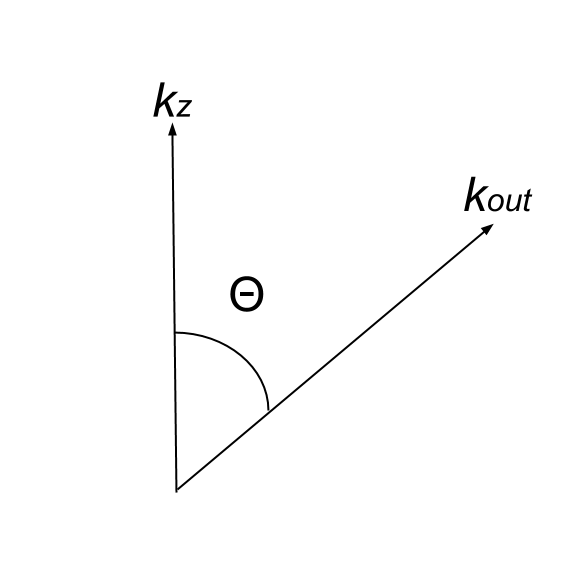
\includegraphics[scale=0.2]{Figures/theta.png}
\end{figure}
\end{frame}

\begin{frame}
\begin{figure}
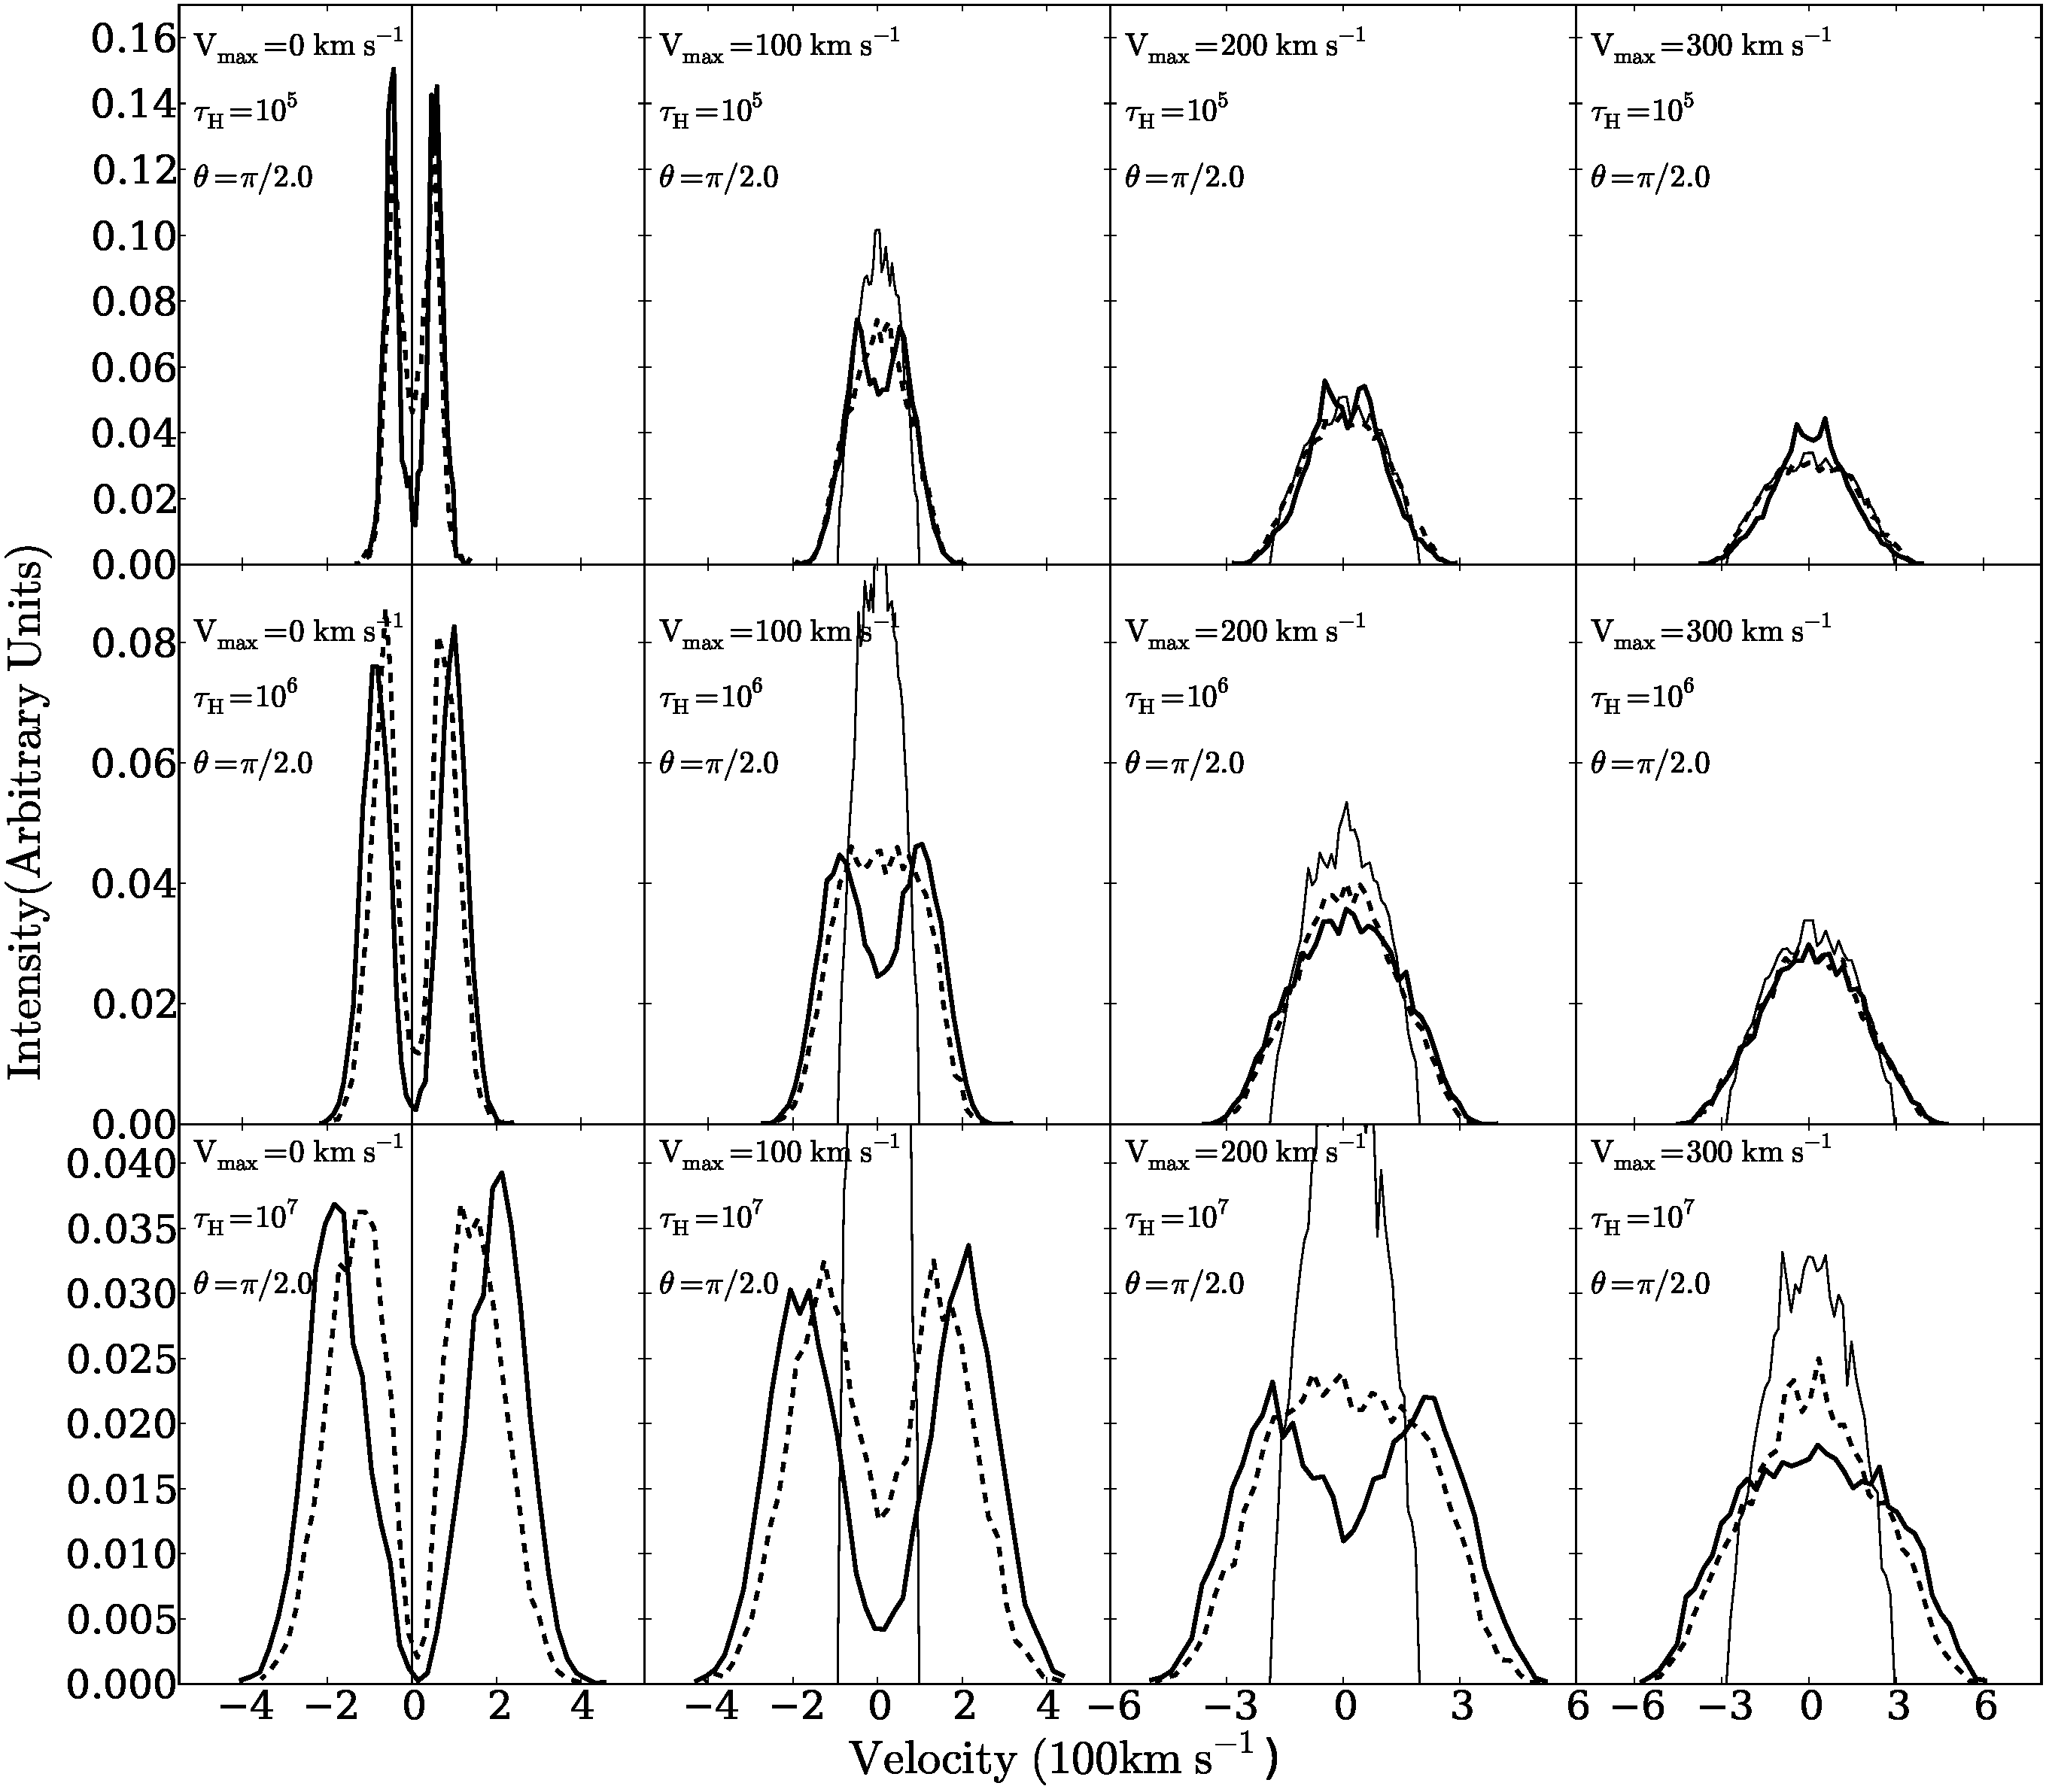
\includegraphics[scale=0.2]{Figures/f4.pdf}
\caption*{Garavito-Camargo e.a 2014}
\end{figure}
\end{frame}

\begin{frame}{Central model spectrum:}
\begin{figure}
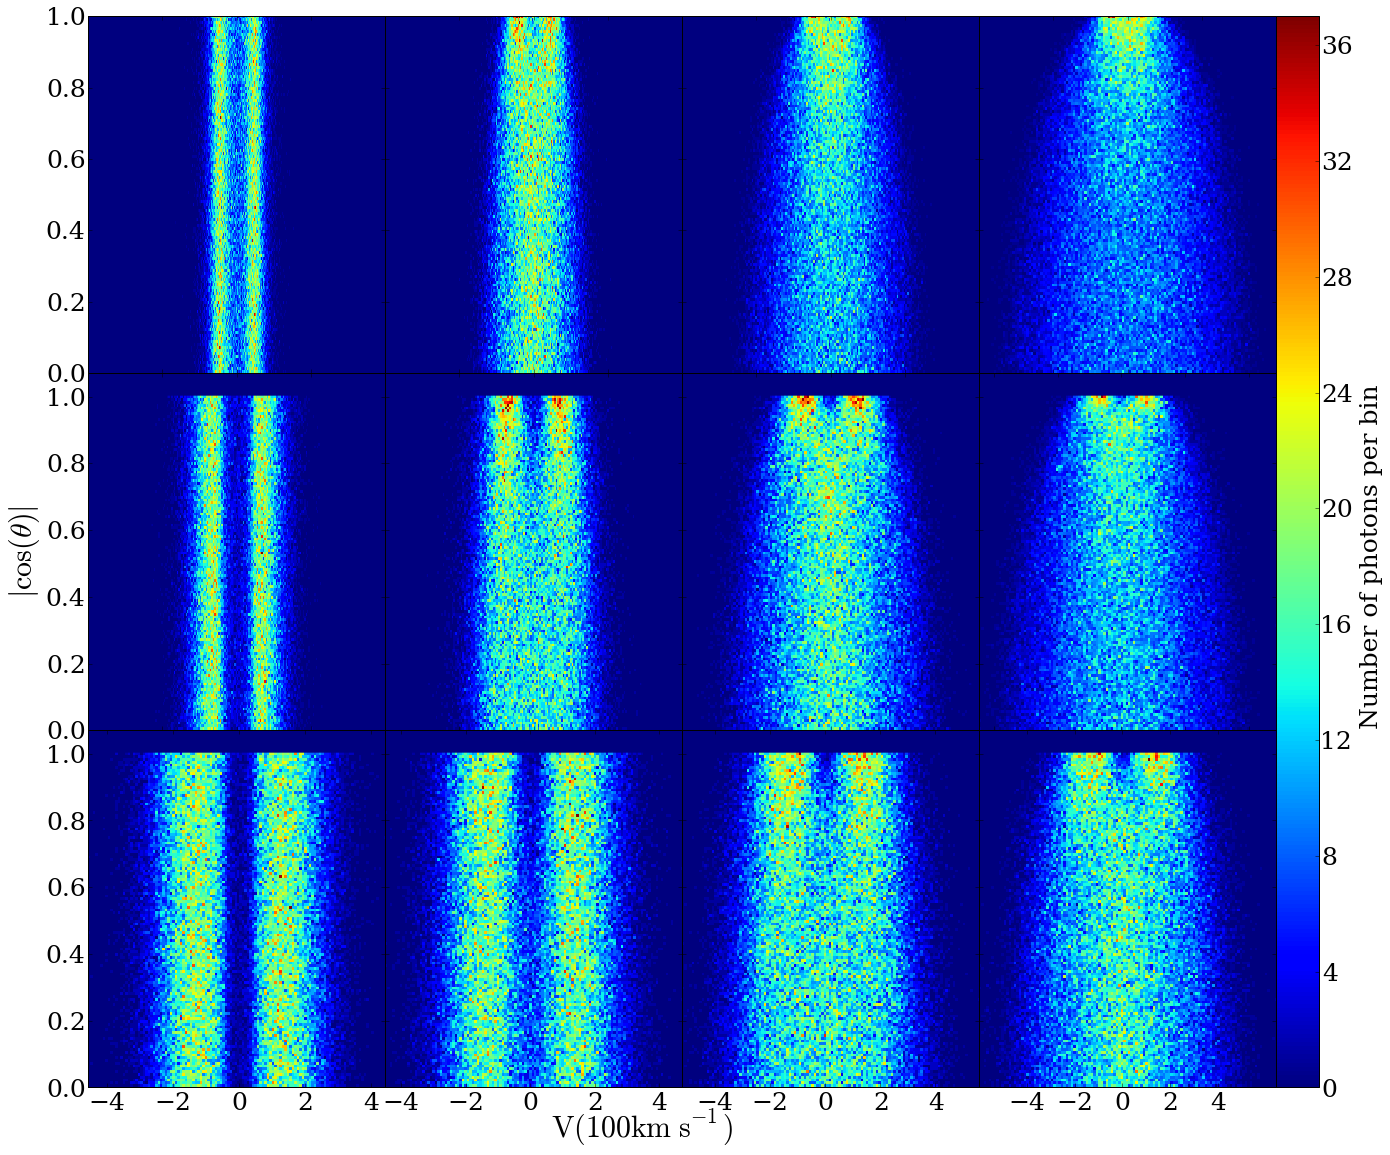
\includegraphics[scale=0.18]{Figures/f2.png}
\caption*{Garavito-Camargo e.a 2014}
\end{figure}
\end{frame}

\begin{frame}{Homogeneous model spectrum:}
\begin{figure}
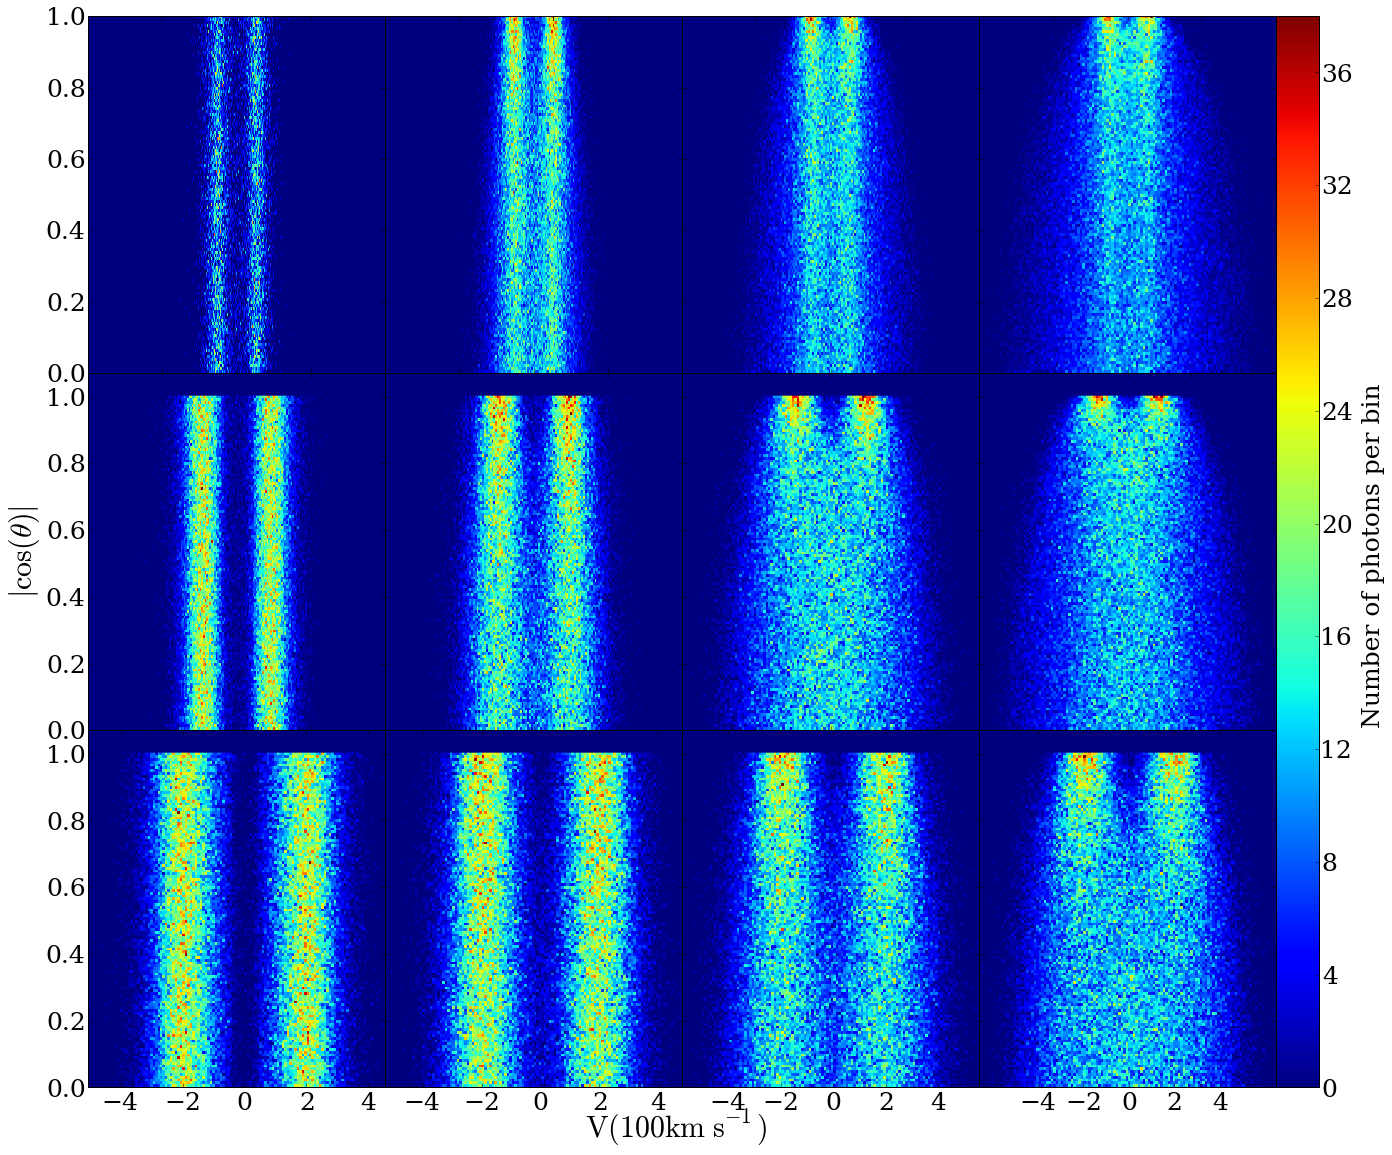
\includegraphics[scale=0.18]{Figures/f3.png}
\caption*{Garavito-Camargo e.a 2014}
\end{figure}
\end{frame}

%\begin{frame}{Simulated spectra}
%\begin{figure}
%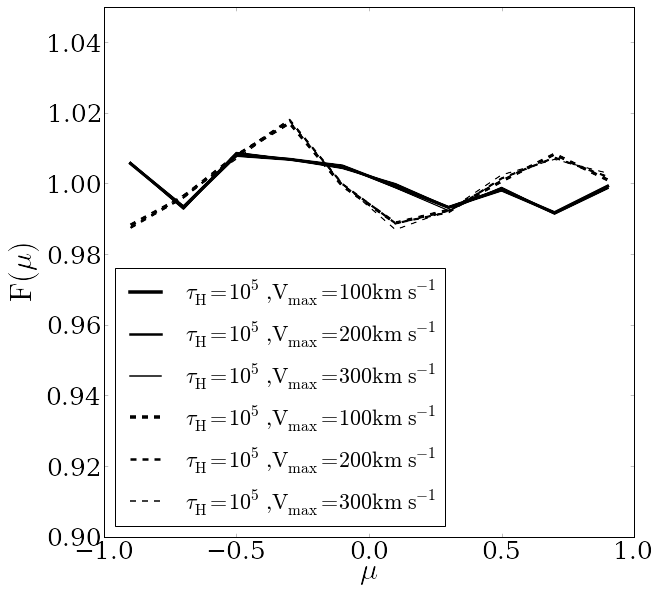
\includegraphics[scale=0.4]{Figures/f5.png}
%\end{figure}
%\end{frame}


\begin{frame}{The width of the line \textbf{increases} proportional to the rotation velocity.}
\begin{figure}
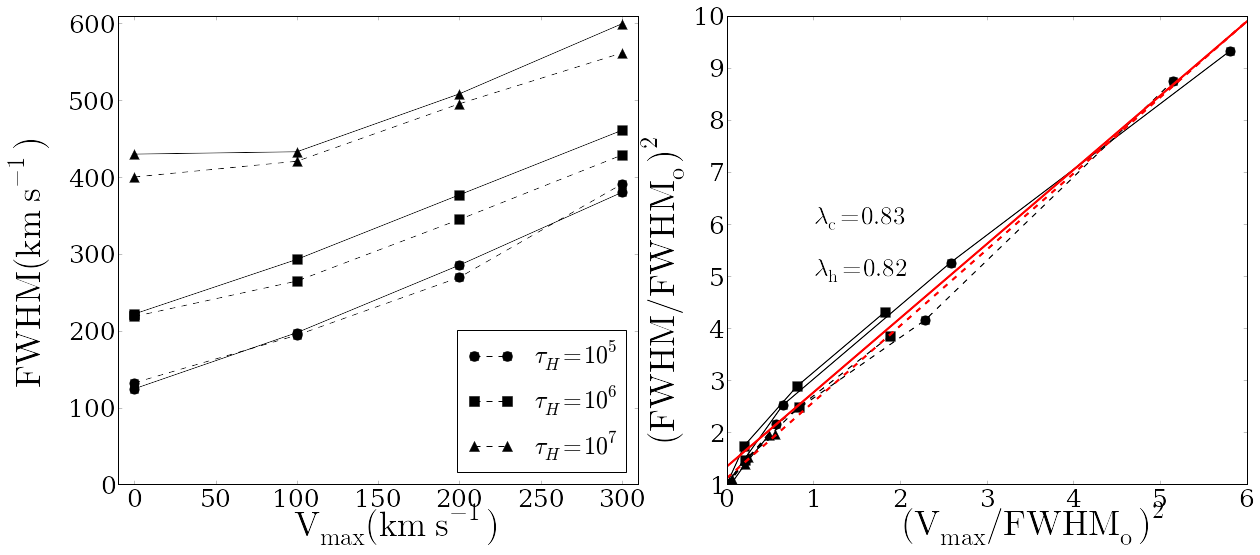
\includegraphics[scale=0.26]{Figures/f7.png}
\caption*{Garavito-Camargo e.a 2014}
\end{figure}
\end{frame}


\begin{frame}{The width of the line \textbf{increases} proportional to the viewing angle $\theta$}
\begin{figure}
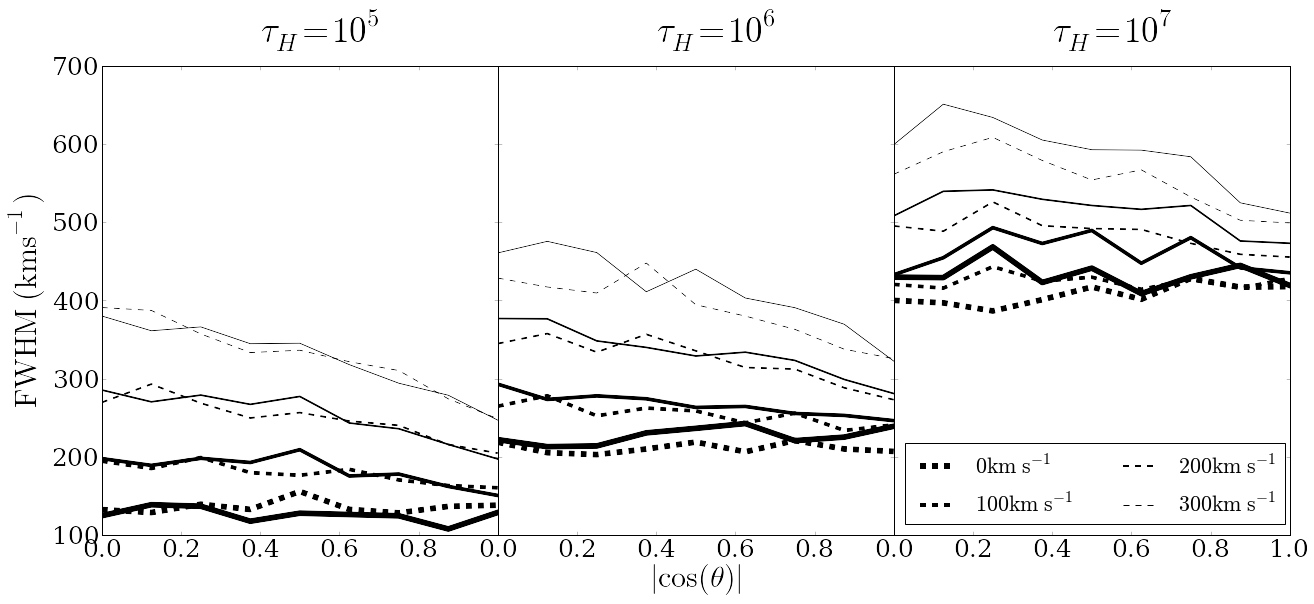
\includegraphics[scale=0.23]{Figures/f6.png}
\caption*{Garavito-Camargo e.a 2014}
\end{figure}
\end{frame}

\begin{frame}{The flux at the line center \textbf{increases} with the rotation velocity and the viewing angle $\theta$.}
\begin{figure}
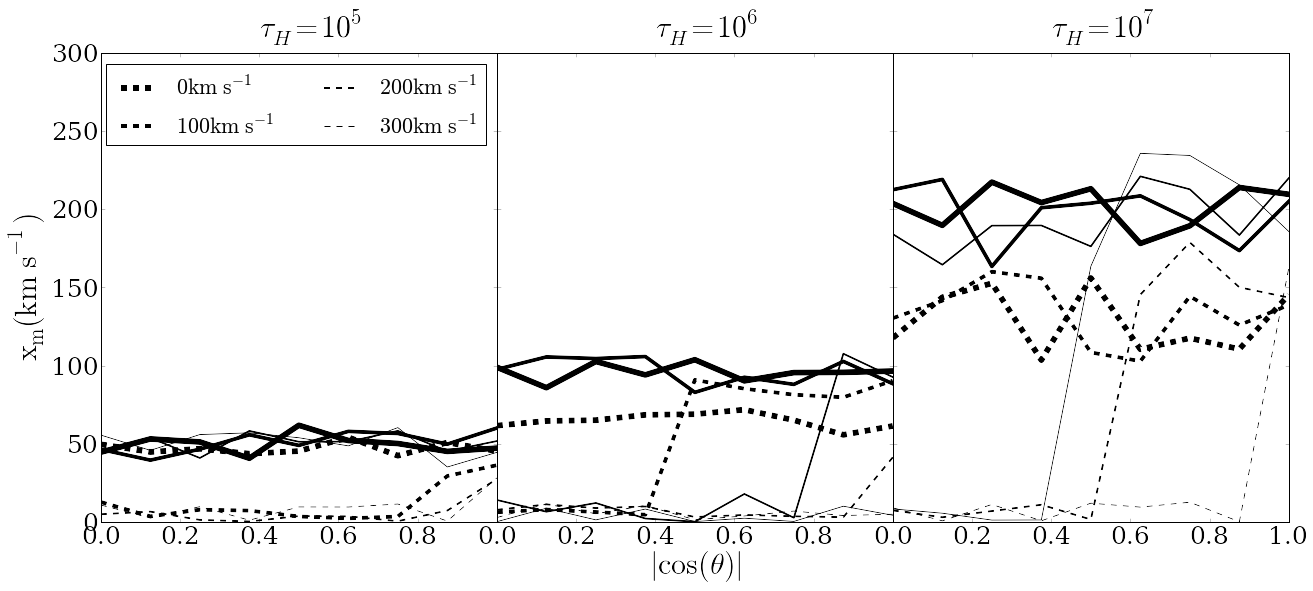
\includegraphics[scale=0.23]{Figures/f8.png}
\caption*{Garavito-Camargo e.a 2014}
\end{figure}
\end{frame}

\begin{frame}{The avergae number of scatterings is \textbf{unaffected} by rotation and viewing angle.}
\begin{figure}
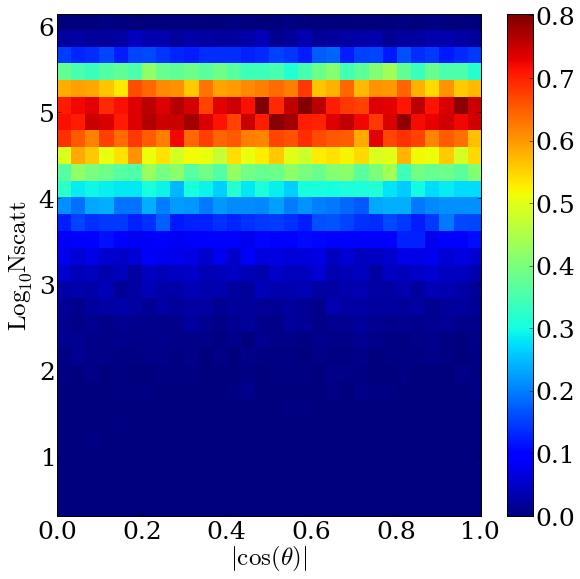
\includegraphics[scale=0.30]{Figures/f9h.png}
\caption*{Garavito-Camargo e.a 2014}
\end{figure}
\end{frame}

\begin{frame}{The escape fraction of Ly$\alpha$ is \textbf{unaffected} by rotation and viewing angle.}
\begin{figure}
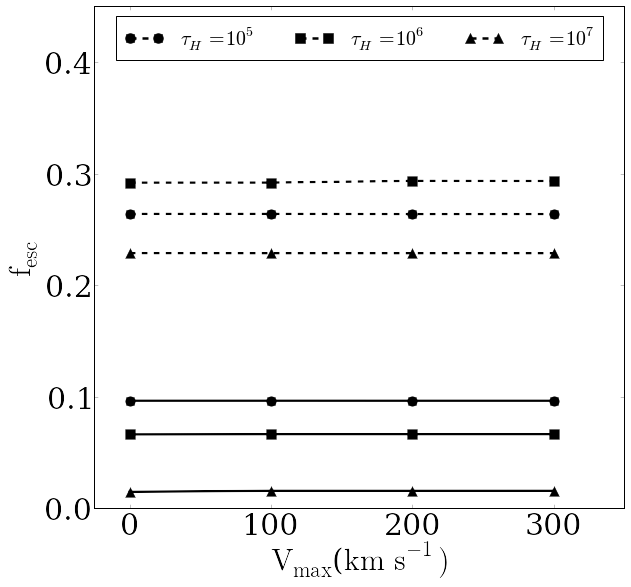
\includegraphics[scale=0.30]{Figures/f10.png}
\caption*{Garavito-Camargo e.a 2014}
\end{figure}
\end{frame}

\begin{frame}{Analytic aproximation}

\begin{equation}
J(x, b, \phi, i) = \dfrac{\sqrt{\pi}}{\sqrt{24}a\tau}\left( \dfrac{(x - x_b)^2}{1 + cosh[\sqrt{\dfrac{2\pi^3}{27}}\dfrac{|(x-x_b)^3|}{a\tau}]} \right ) 
\end{equation}


\begin{equation}
J(x, i) = 2\pi \int \limits_0^R db b \int \limits_0^{2\pi}d\phi S(b,\phi)J(x, b, \phi, i) \approx 2\pi \int \limits_0^R db b \int \limits_0^{2\pi}d\phi J(x, b, \phi, i)
\end{equation}
\end{frame}

\begin{frame}
\begin{figure}
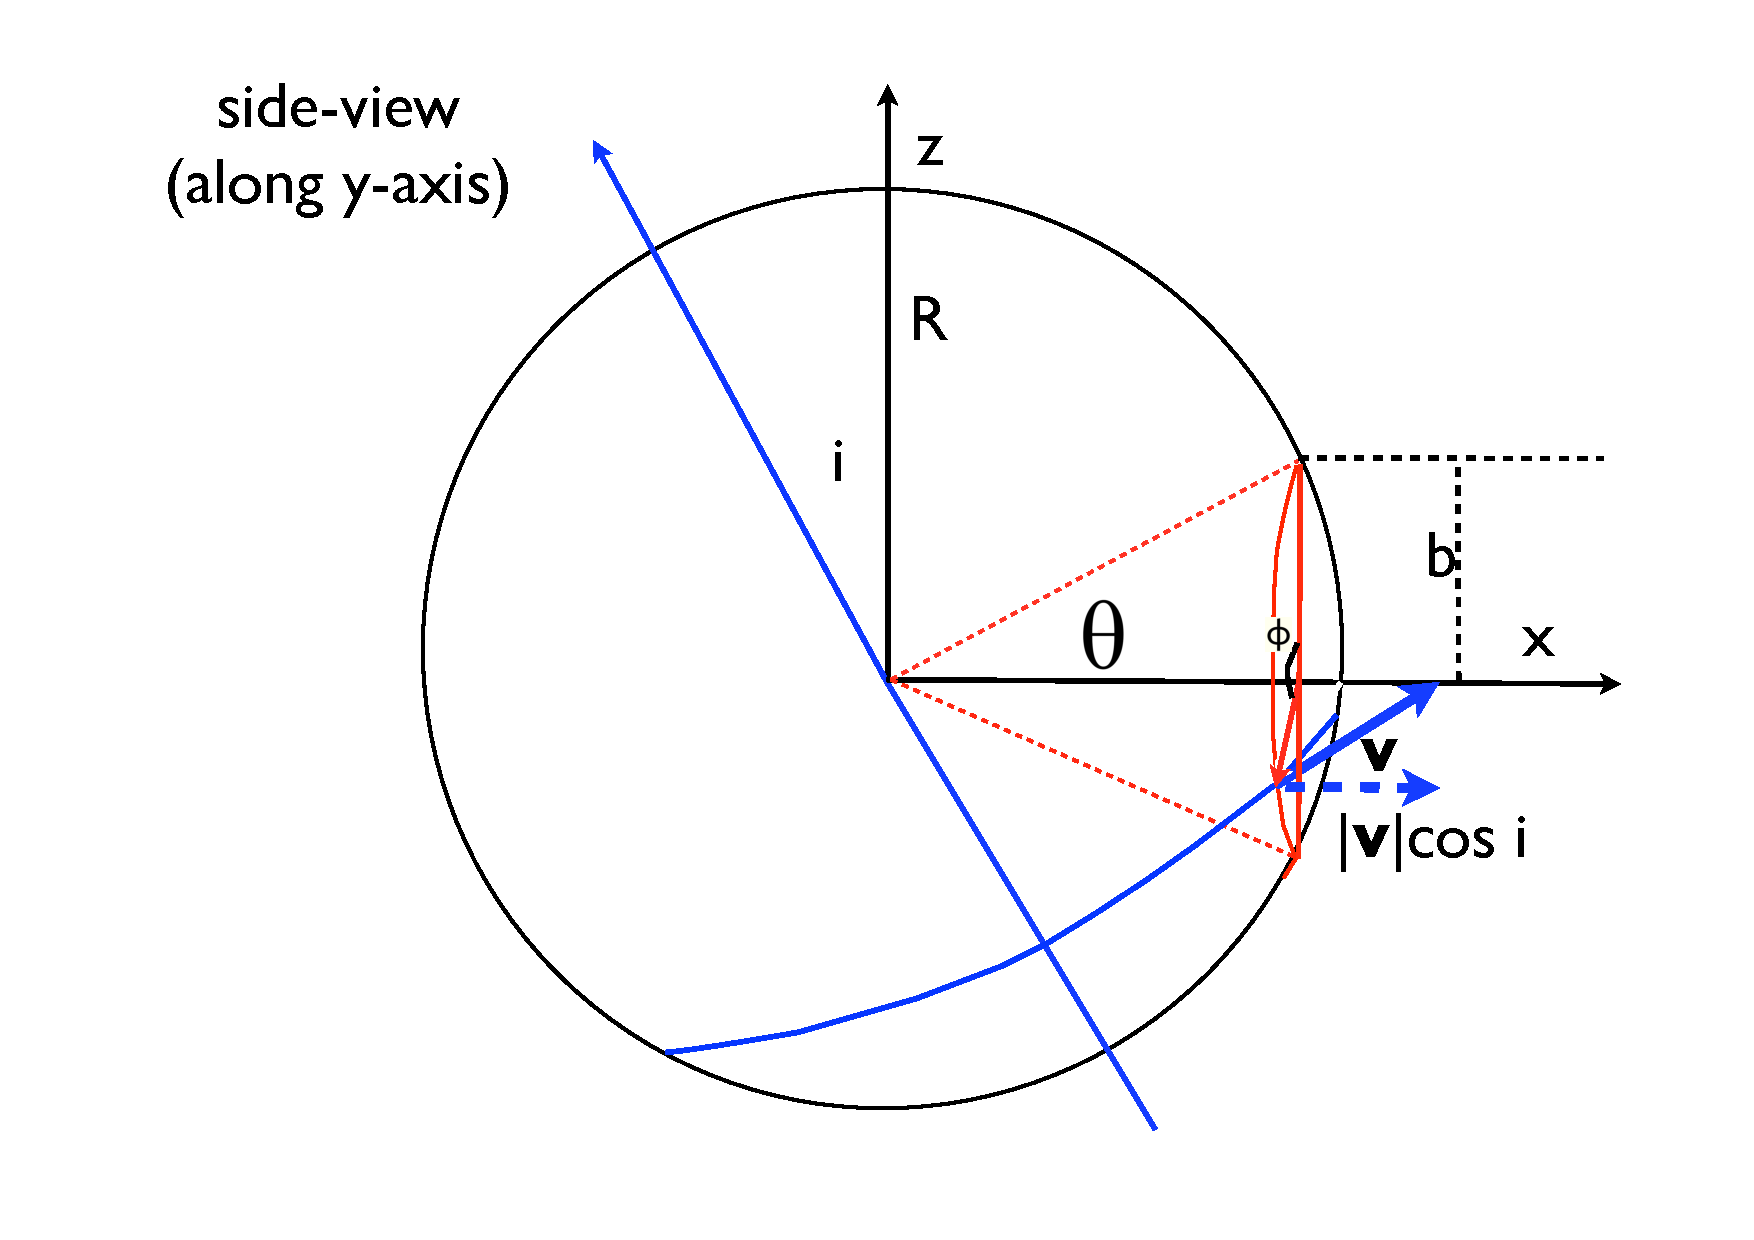
\includegraphics[scale=0.2]{Figures/fig11a.pdf}
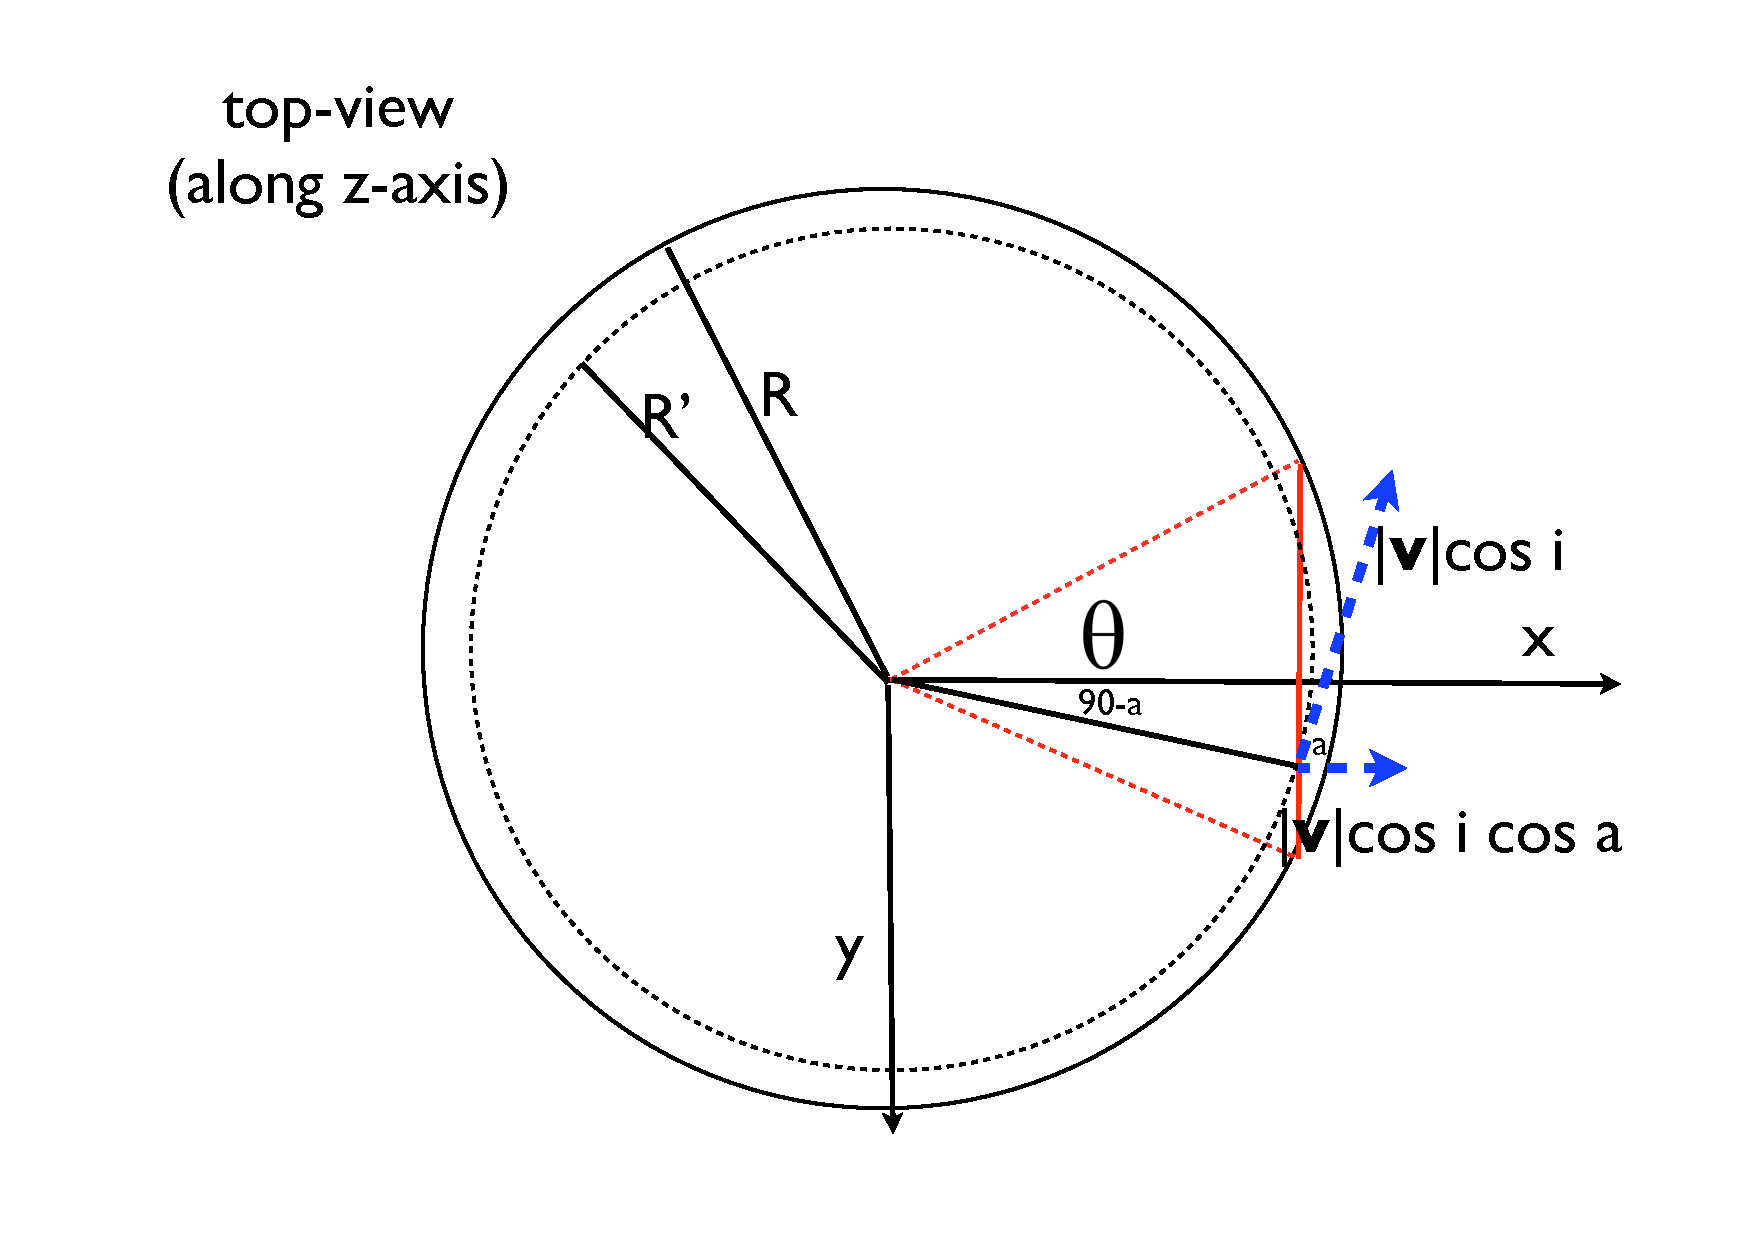
\includegraphics[scale=0.2]{Figures/fig11b.pdf}
\caption*{Garavito-Camargo e.a 2014}
\end{figure}

\begin{equation}
v_b(b, \phi, i) =   V_{max}\dfrac{\sqrt{R^2 - s^2}}{R}cosi cosa
\end{equation}

\begin{equation}
tan \beta = tan|90^o-a| = \dfrac{c}{d} = \dfrac{b sin \phi}{\sqrt{R^2 - b^2}}
\end{equation}
\end{frame}

\begin{frame}{Analytic aproximation}
\begin{figure}
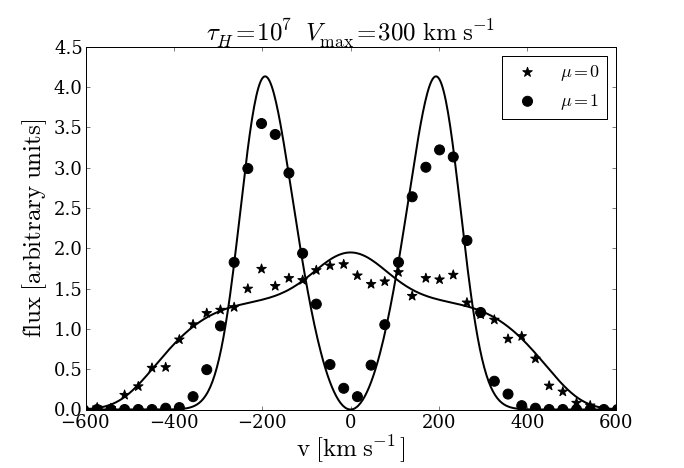
\includegraphics[scale=0.2]{Figures/vary_angle1.png}
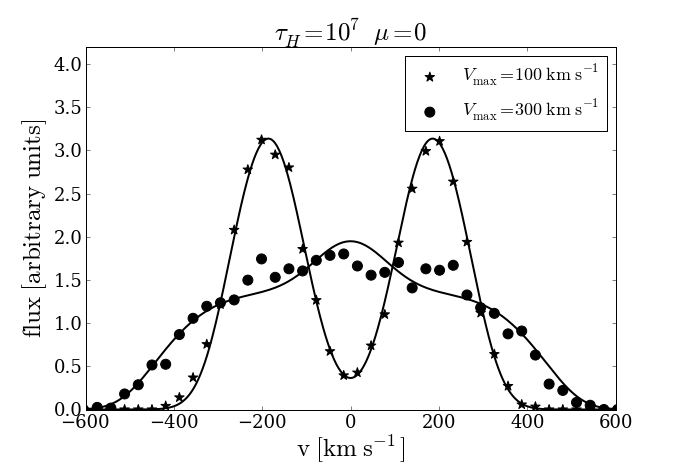
\includegraphics[scale=0.2]{Figures/vary_vel1.png}
\caption*{Garavito-Camargo e.a 2014}
\end{figure}
\end{frame}



\begin{frame}{Lyman alpha observed in rotation}
\begin{figure}
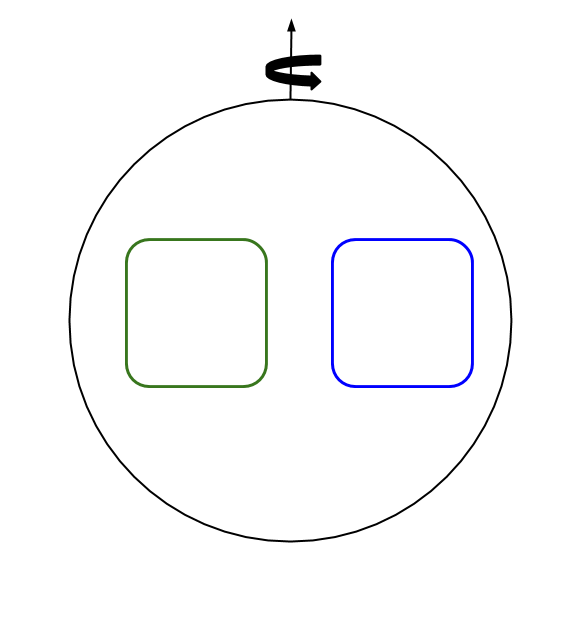
\includegraphics[scale=0.2]{Figures/measure.png}
\end{figure}
\end{frame}

\begin{frame}{Conclusions:}
\textbf{1.} Rotation has an impact in the Ly$\alpha$ line morphology; the width and the relative intensity 
of the peaks and the center of the line are affected.  For high velocities the line broadens and
becomes single peaked. This boradens follows:

\[
FWHM^2 = FWHM_0^2 + \left( \dfrac{V_{max}}{\gamma} \right )^2
\]
\end{frame}

\begin{frame}{Conclusions:}
\textbf{2.} Rotation induces an anisotropy for different viewing angles, for viewing angles close to the 
pole the line are double peaked and the line makes a transition to single peaked for viewing 
angles along the equator.
\end{frame}


\begin{frame}{Conclusions:}
\textbf{3.} The scape fraction $f_{esc}$, the average number of scatterings $N_{scatt}$ 
and the integrated flux of the line are not affected by rotation neither by the viewing angle.
\end{frame}

\begin{frame}{Work in progress}
Fit of the line
\end{frame}

\begin{frame}{Work in progress}
rotation + outfloes
\end{frame}

\end{document}
